\section{Оптимальные значения}

\subsection{Рассмотрим игру за преподавателя}
\begin{flushleft}

	Игрое \textbf{П} стремится минимизировать функциональный критерий: 
	
	$$F(x, y) = (\frac{y\sqrt{x}}{2},\frac{\sqrt{1-x}}{y})$$	

	Игрок \textbf{П} использует смешанную стратегию, т.е. его стратегией является
	распределение $p=(p_0,p_1)$ над множеством чистых стратегий $Y=\{1,2\}$:\\
	
	$$
	F_\textrm{П}(p,x)=
	\big \langle 
		(1-p)\frac{1 \cdot \sqrt{x}}{2} + p \frac{2 \cdot \sqrt{x}}{2}; \;
		(1-p)\frac{\sqrt{1-x}}{1}+p\frac{\sqrt{1-x}}{2} 
	\big \rangle=
	\frac{1}{2}
	\big \langle
		(p+1)\sqrt{x}; \;
		(2-p)\sqrt{1-x}
	\big \rangle
	$$
	
	Затем использует \textbf{ЛС} (1):
	
	$$
	L(p,x,\lambda)=
	\frac{1}{2}
	\big(
		\lambda(p+1)\sqrt{x} + (1-\lambda)(2-p)\sqrt{1-x}
	\big)
	$$
	
	Введём обозначение $q=(q_0,q_1,q_2)$. Далеем осредняем 
	функцию $L(p,x,\lambda)$ по стратегиям противника $x \in X=\{0,\frac{1}{2},1\}$ c 
	вероятностями $q=(q_0,q_1,q_2)$:
	
	\begin{gather*} 
	\overline{L}(p,q,\lambda)=
	\frac{1}{2} 
	\Big(
		q_0(1-\lambda)(2-p)\sqrt{1}+
		q_1 \big (\lambda(p+1)\frac{1}{\sqrt{2}} + 
		(1-\lambda)(2-p)\frac{1}{\sqrt{2}} \big )+
		q_2\lambda(p+1)\sqrt{1}
	\Big)=
	\\
	=\frac{1}{2\sqrt{2}}
	\Big (
		\big (\lambda(q_1+\sqrt{2}q_2)-(1-\lambda)(q_1+\sqrt{2}q_0) \big)p+
		\big (\lambda(q_1+\sqrt{2}q_2)+2(1-\lambda)(q_1+\sqrt{2}q_0) \big)
	\Big)
	\end{gather*}
	
	Функция является линейной по переменной $p$:
	
	$$
	\overline{L}(p,q,\lambda)=k(\lambda,q)p+b(\lambda,q)
	$$
	где
	$$
	k(q, \lambda) = \frac{1}{2\sqrt{2}}
		\big (\lambda(q_1+\sqrt{2}q_2)-(1-\lambda)(q_1+\sqrt{2}q_0) \big)
	$$
	$$
	b(q, \lambda) = \frac{1}{2\sqrt{2}}
		\big (\lambda(q_1+\sqrt{2}q_2)+2(1-\lambda)(q_1+\sqrt{2}q_0) \big)
	$$
	
	Наша задача найти 
	$p^*(q, \lambda)=\arg \min \limits_{p \in [0, 1]} \overline{L}(p,q,\lambda)$.
	Поскольку функция $\overline{L}(p,q,\lambda)$ линейна по переменной 
	$p$, следовательно:
	
	$$
		p^*(q, \lambda)=
		\arg \min \limits_{p \in [0, 1]} \overline{L}(p,q,\lambda)=
		\begin{cases}
			0, & k(\lambda,q)>0 \\
			1, & k(\lambda,q)<0 \\
			[0,1], & k(\lambda,q)=0
		\end{cases}	
	$$
	
	Рассмотрим функцию $k(q, \lambda)=\frac{1}{2\sqrt{2}}
	\Big(
		\lambda \big (2+(\sqrt{2}-2)(q_0-q_2) \big) -
		\big (1 - q_2 + (\sqrt{2} - 1)q_0 \big)
	\Big)
	$

	Нас интересует знакт это функции при различных значениях аргументов.
	Введём обозначения:
	
	$$\ell(q) = \frac{1 - q_2 + (\sqrt{2} - 1)q_0}{2+(\sqrt{2}-2)(q_0-q_2)}$$	
	
	Напомним, что множестово $Q$ имеет следующий вид:
	$$
		Q=\{(q_0,q_2) \in \mathbb{R}^2 \; | \;
		0 \leqslant q_i \leqslant 1 \; i\in\{0,2\}; \; 
		q_0 + q_2 \leqslant 1\}	
	$$	
	
	Поскольку для $q \in Q$ верно: 
	\begin{gather*}
	2+(\sqrt{2}-2)(q_0-q_2) > 0 \\
	1 - q_2 + (\sqrt{2} - 1)q_0 \geqslant 0 \\
	q_0 + (\sqrt{2} - 3) q_2 - 1 \leqslant 0 \\
	\end{gather*}
	
	Следовательно:
	
	$$
	k(q, \lambda) \vee 0 \Leftrightarrow 
	\lambda \vee \ell(q) \textrm{ где } \vee \textrm{ это один из знаков } >,<,=.
	$$
	
	Более того верно что 
	$\forall q \in Q \; 0 \leqslant \ell(q) \leqslant 1$. 
	Проиллюстрируем это на графике. В плоскости $q=(q_0,q_2)$ изображены 
	прямые $\ell_1(q)$ и $\ell_2(q)$ такие, что:
	$$\ell_1(q): \; \ell(q)=0 $$
	$$\ell_2(q): \; \ell(q)=1 $$
		
	зелёным цветом изображена область в которой
	$0 \leqslant \ell(q) \leqslant 1$.
	Видно, что квадрат $q = [0,1]^2$ а следовательно и
	множетсво $Q$ полностью принадлежит этой области.

	\begin{figure}[H]
		\centering
  		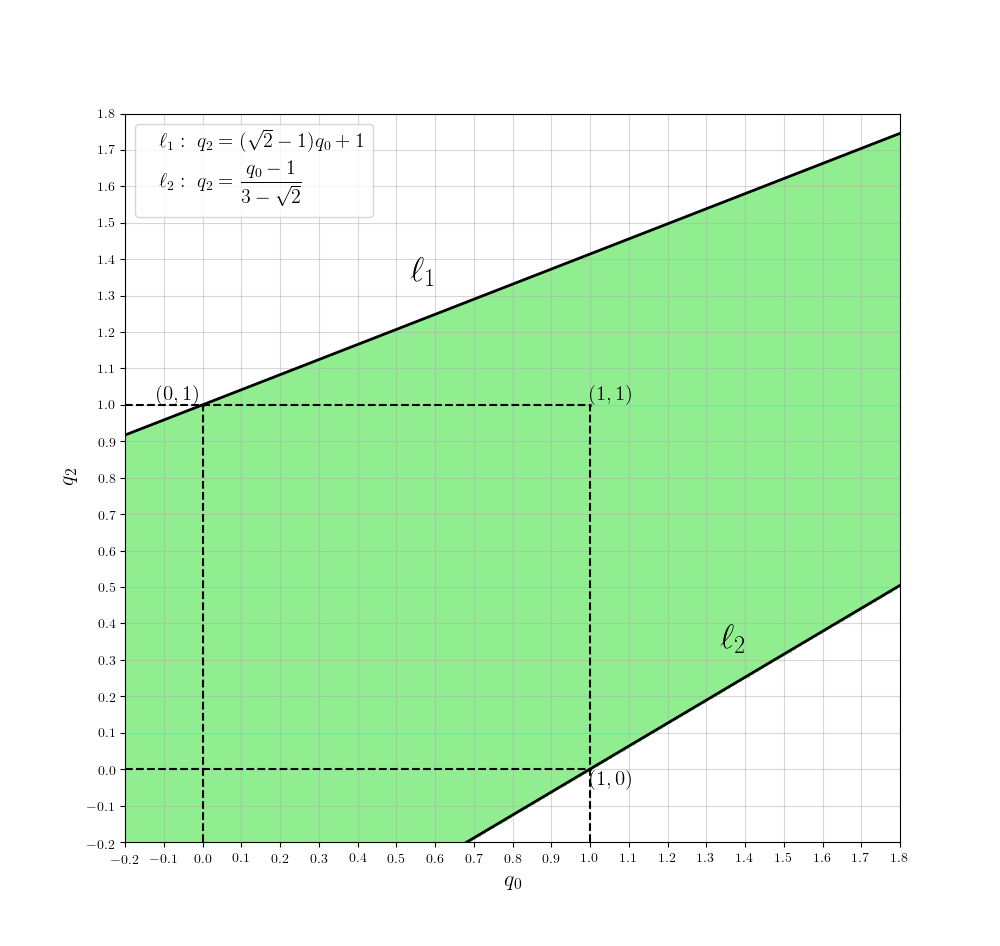
\includegraphics[scale=0.4]{part_3/graf_3_1}
  		\caption{}
	\end{figure}
	
	Следовательно $\forall q=(q_0, q_2) \in Q \;
	\exists \; \lambda \in [0,1]: \; k(\lambda,q)=0$.
	
	$$
		p^*(\lambda,q)=
		\arg \min \limits_{p \in [0, 1]} \overline{L}(p,q,\lambda)=
		\begin{cases}
			0, & \lambda \in \big(\ell (q), 1\big] \\
			1, & \lambda \in \big[0, \ell(q) \big) \\
			[0,1], & \lambda=\ell(q)
		\end{cases}
		\textrm{ , где } \ell(q)=
		\frac{1 - q_2 + (\sqrt{2} - 1)q_0}{2+(\sqrt{2}-2)(q_0-q_2)}
	$$	
	
\end{flushleft}